\documentclass[a4paper]{article}
\usepackage{a4wide}
% \usepackage{graphicx}
% \usepackage{amssymb,amsmath}
% \usepackage{booktabs}
\usepackage[english]{babel}
% \usepackage{multirow}
\usepackage{graphicx}% Include figure files
% \usepackage{color}
\emergencystretch=35pt
\usepackage[pdftex,unicode,colorlinks, citecolor=blue,%
filecolor=black, linkcolor=blue, urlcolor=black]{hyperref}
\usepackage[figure,table]{hypcap}


\begin{document}
\begin{center}
  Response Letter
\end{center}
Dear Editor,
\vspace{10pt}

Many thanks for sending us referees’ reports on our manuscript
entitled “Superabsorption of light by nanoparticles” by K. Ladutenko
et al. (editorial code NR-COM-08-2015-005468). We are pleased with
overall very positive tone of these reports, as well as with referees’
constructive comments.

We have addressed all the comments of the referees, and we present our
response and the summary of the changes made to the manuscript below.
\vspace{10pt}
\\
Sincerely Yours,\\
On behalf of the authors,\\
Konstantin Ladutenko


\vspace{10pt}

\newpage
\textbf{Reviewer \#1 comments}

\begin{tabular}[!H]{l|p{0.9\textwidth}}
\quad & 1. The authors claimed “Combined effect of these resonances is
presented to produce the flat and relative broadband electric
resonance response.” Nevertheless, the broadened absorption band is
not very broad. Is there any further way to predict a broadband light
absorption. For instance, a broadband absorption in the whole visible
spectral range. Maybe, a possible way of using the dispersed size
scale nanoparticles should be added for improving the study.
\end{tabular}\\

We thank the referee for suggestion. First, we would like to note that
the term "broadband" is quite loose, when not defined explicitly. For
example, if we compare our absorption band with the whole C-band of
the optical fibres, which is used to carry Terabits of data, and which
is just 35 nm wide, then our absorbers are extremely broadband, since
they have the bandwidth approaching 100 nm. Compared to the whole
visible spectrum, however, indeed our absorption band is not very
broad. So, to address the referee comment, we decided to study the
possible ways to enhance the width of the absorption band.

We can think of a two possible approaches to achieve the broadband
performance. First approach utilizes the mix of different particles,
while the second approach uses several resonances within one
particle. The later approach is nontrivial and requires large
additional study, that would deserve a separate publication. The first
approach, however, mentioned by the Referee, is more straightforward,
and we can use a mixture of different particles, so that particles of various sizes absorb different wavelengths.  To illustrate this we have
run an optimization procedure to find two designs: one absorbs at
475~nm, while another is centered at 525~nm (outer radii 34 and 38~nm,
respectively). We then combine such particles to form a dimer, and
calculate its properties using Lumerical FDTD Solutions. Sketch of the
simulated system and final results are shown in
Fig.~\ref{fig:fdtd}. As a reference, we also perform FDTD simulations
of standalone spheres, and the obtained positions and we found that the amplitudes of
resonances match well the results of the Mie calculations.
\begin{figure}
  \begin{minipage}[h]{0.49\textwidth}    \begin{flushleft}     a)    \end{flushleft}
  \end{minipage}
  \begin{minipage}[h]{0.49\textwidth}    \begin{flushleft}     b)    \end{flushleft}
  \end{minipage}
  \begin{minipage}[h]{0.49\textwidth} 
   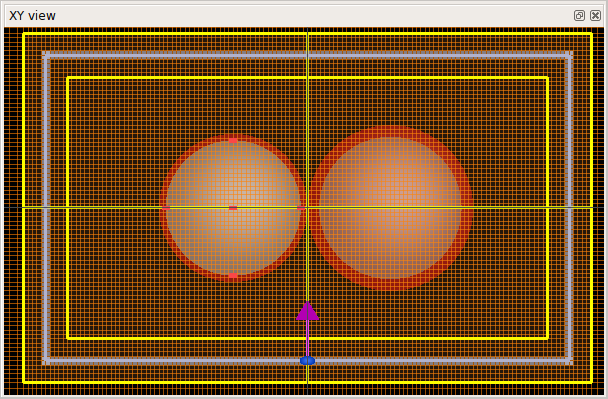
\includegraphics[width=0.95\textwidth]{FDTD-mode-d00}
  \end{minipage}
  \begin{minipage}[h]{0.49\textwidth} 
   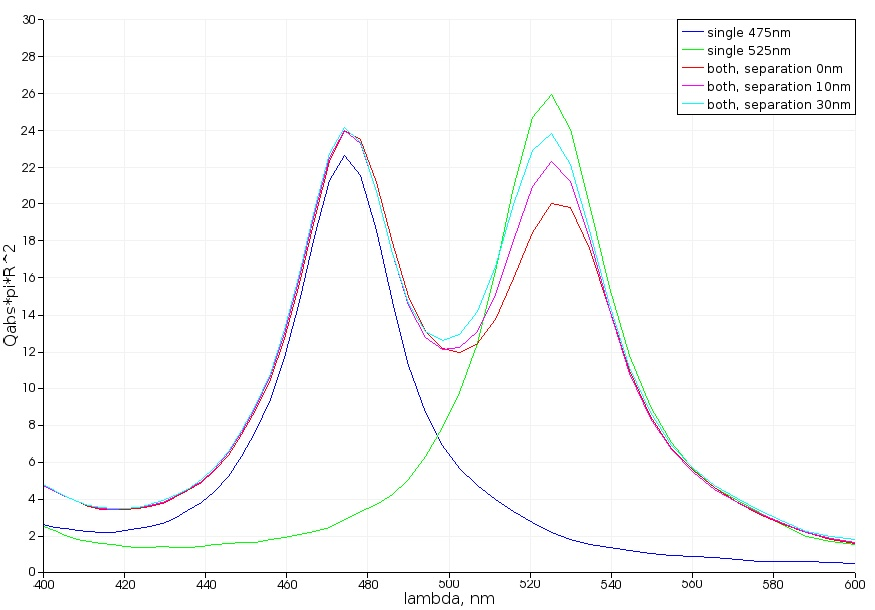
\includegraphics[width=0.95\textwidth]{fdtd-spectra}
  \end{minipage}
  \begin{minipage}[h]{0.49\textwidth}    \begin{flushleft}     c)    \end{flushleft}
  \end{minipage}
  \begin{minipage}[h]{0.49\textwidth}    \begin{flushleft}     d)   \end{flushleft}
  \end{minipage}
  \begin{minipage}[h]{0.49\textwidth} 
    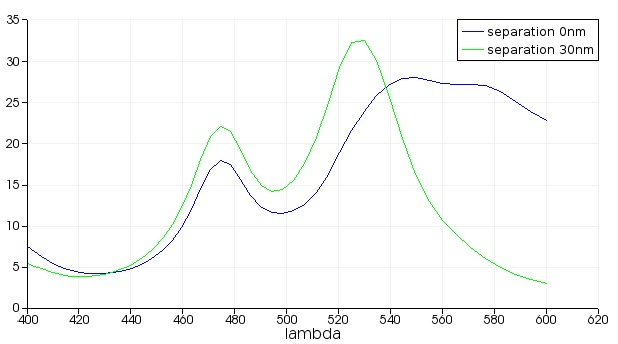
\includegraphics[width=0.95\textwidth]{fdtd-spectra-Ek}
  \end{minipage}
  \begin{minipage}[h]{0.49\textwidth} 
    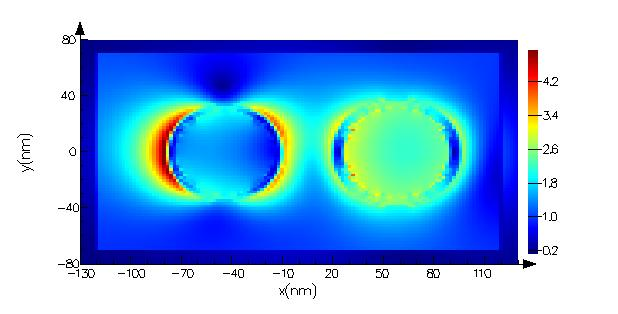
\includegraphics[width=0.95\textwidth]{fdtd-field}
  \end{minipage}
    \caption{(a) Sketch of the simulated dimer in full wave
      simulations by Lumerical FDTD. (b) Absorption spectra of
      stand-alone spheres and in dimer configuration with separation
      between spheres of 0, 10, and 30~nm, particles are in H-k plane;
      (c) Separation 0 and 30~nm for particles in E-k plane; (d) Field
      distribution for the incident wavelength of 500 nm for particles
      in E-k plane with separation of 30~nm.\label{fig:fdtd}}%
\end{figure}

When we mix the different sized spheres, there will be an effect of
their mutual interaction. To take this into account, we simulate a
dimer configurations with 0 nm, 10 nm and 30 nm separation between
spheres.  The resulting spectra have a strong contribution from
standalone resonances, while coupling effects seems to be relatively
minor. This can be explained from modal field distribution in
Fig.~4(c) of the manuscript. Positioning spheres in H-k plane we are
exploiting the fact that the fields are highly localized inside the
spheres. Arranging spheres in other planes with respect to incident
polarization, or increasing the number of interacting spheres can
change the effect of coupling. As an example, we tested arrangement of
spheres in E-k plane Fig.~\ref{fig:fdtd}(c); for zero separation the
interaction between spheres is strong, however, due to near-field
nature of this coupling, it rapidly decays with the separation width
Fig.~\ref{fig:fdtd}(d), for separation of 30~nm responses of
individual particles dominate in overall spectra for both planes of
polarization. This way we show that in principle it is possible to
construct an absorption band of an array of dispersed particles simply
optimizing the properties of individual particles.

In order to reflect these findings in the manuscript, we have
rewritten the text from ``As a result, one can design
spectrally-selective absorbers or broadband absorbers with almost
arbitrary prescribed properties.'' to ``As a result, one can design
absorbers with broad spectra or spectrally-selective absorbers with
almost arbitrary prescribed properties.  One can also achieve
broadband performance by mixing particles whose absorption is
optimized for different wavelengths. We have verified that due to
strong localization of electric dipole field it is possible to design
dimers whose absorbing properties are dominated by the properties of
individual particles, and not by their mutual interaction. As a
result, by appropriately spacing the resonances of individual
particles, their mixture will exhibit a combined broadband
response. Providing such an additional control, this approach
complements the case of self-organized particles of various size and
shape, which was experimentally proved to have a wide absorption
band~[ACS-AMI-Liu-2015]. % Reference to the paper mentioned with the
% reviewer in his second comment.
Further control of the absorption spectrum can be achieved by
arranging our spherical structures in a periodic and non-periodic
arrays.''

\begin{tabular}[!H]{l|p{0.9\textwidth}}
  \quad & 2. To achieve super-absorption behavior, it is interesting
  to know what will happen when the multilayered nanoparticles are
  closely packed as the plasmonic crystal. As reported in the previous
  papers [ACS Applied Materials \& Interfaces, 7, 4962−4968 (2015);
  Materials Letters 158, 262–265 (2015); Applied Physics Letters, 104,
  081116 (2014); Nanotechnology, 24, 155203 (2013)], the packed
  plasmonic crystals have been demonstrated to show broadband light
  coupling and confinement. Thereby, it would be interesting to show
  improved broadband light absorption based on the plasmonic crystal
  of this proposed multilayered nanoparticles. 
\end{tabular}

We would like to thank the reviewer for the references. We have
included them into our manuscript with relevant discussions,
% ACS-AMI was added to reply on the previous comment, ML and NT can be added to
% the links on plasmonic devices in introduction along with [19,20].
with one exception. Reference Applied Physics Letters, 104, 081116
(2014) with the title "$\lambda^3$/20000 plasmonic nanocavities with
multispectral ultra-narrowband absorption for high-quality sensing''
is not related to broadband light coupling and confinement'' and was
probably listed by an accident.

We agree with the referee that closely packed particles can lead to
the increase of the bandwidth. This broadening originates from the
appearance of a collective mode (or, in other words, the hybridization
of plasmon responses of several particles) with additional impact from
retardation effects. While for some resonances, as we have discussed
in the response to the previous comment, the interaction between our
nanoparticles can be weak, it should still be possible to optimize
simultaneously the geometry of individual particles and the array
parameters to achieve enhanced absorption. As a proof of concept, we
performed FDTD simulations of the 3x3 square array of spheres (to
provide a good coupling both in E and H directions) with the
separation of 4~nm, see Fig~\ref{fig:fdtd-3x3}(a). Several collective
modes can be recognized from field distribution while changing the
incident wavelength Fig~\ref{fig:fdtd-3x3}(c-e). We see that for the
used materials, nanoparticle and array designs, spectral range, and
plane of polarization, we observed a broadened resonance, with the
broadening mostly occurring in the blue shift direction
Fig~\ref{fig:fdtd-3x3}(b).

We believe that the detailed study of the effect of arranging the
elements in array is a whole new project, and it lies outside the
scope of our current manuscript. We have mentioned, however, in the
revised manuscript that further control of the absorption spectrum can
be achieved by arranging our spherical structures in a periodic and
non-periodic arrays.

\begin{figure}
  \begin{minipage}[h]{0.49\textwidth}    \begin{flushleft}     a)    \end{flushleft}
  \end{minipage}
  \begin{minipage}[h]{0.49\textwidth}    \begin{flushleft}     b)    \end{flushleft}
  \end{minipage}
  \begin{minipage}[h]{0.49\textwidth} 
   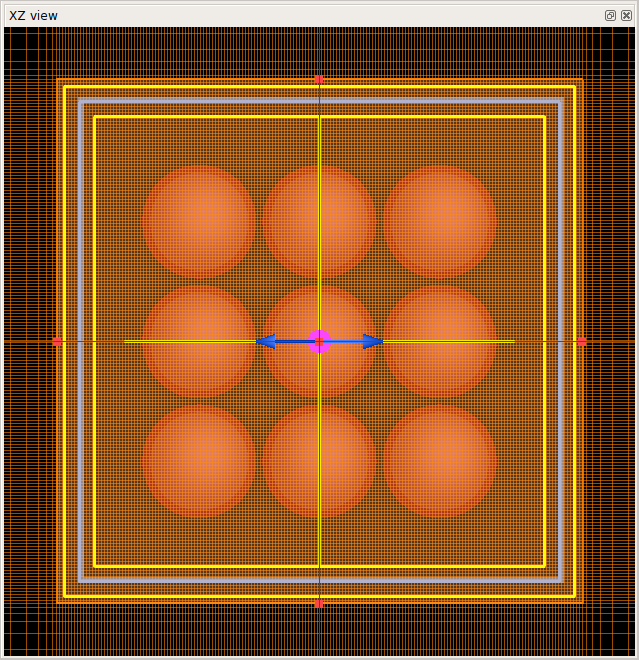
\includegraphics[width=0.95\textwidth]{fdtd-3x3}
  \end{minipage}
  \begin{minipage}[h]{0.49\textwidth} 
   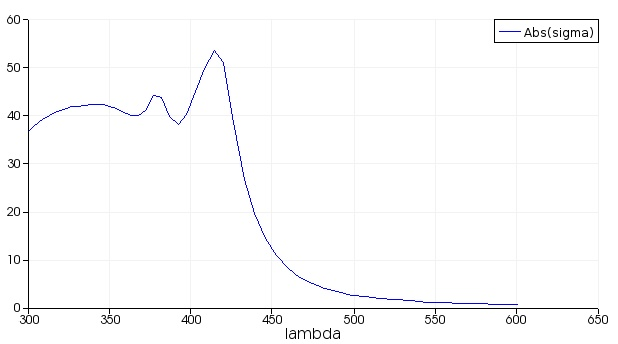
\includegraphics[width=0.95\textwidth]{fdtd-spectra-3x3}
  \end{minipage}
  \begin{minipage}[h]{0.49\textwidth}    \begin{flushleft}     c)    \end{flushleft}
  \end{minipage}
  \begin{minipage}[h]{0.49\textwidth}    \begin{flushleft}     d)   \end{flushleft}
  \end{minipage}
  \begin{minipage}[h]{0.49\textwidth} 
    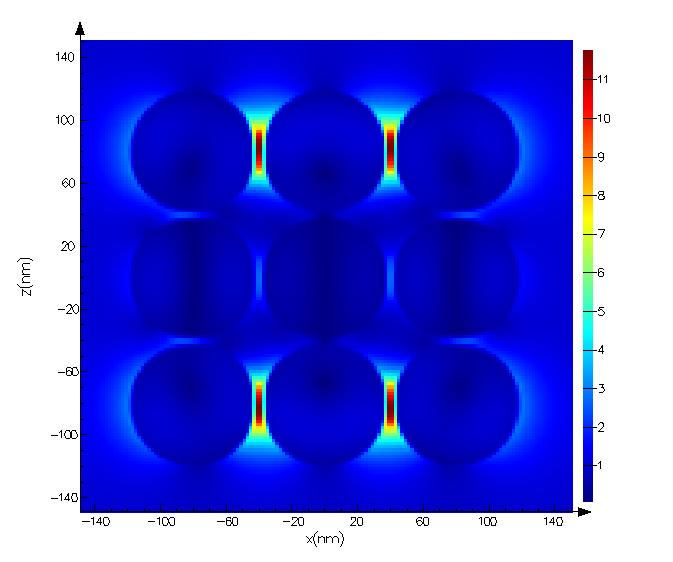
\includegraphics[width=0.95\textwidth]{fdtd-field-408nm}
  \end{minipage}
  \begin{minipage}[h]{0.49\textwidth} 
    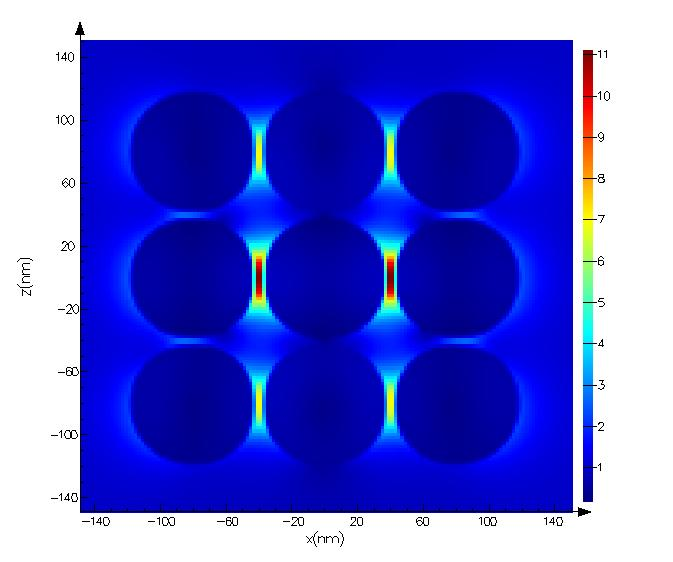
\includegraphics[width=0.95\textwidth]{fdtd-field-452nm}
  \end{minipage}
  \begin{minipage}[h]{0.49\textwidth}    \begin{flushleft}     e)    \end{flushleft}
  \end{minipage}
  \begin{minipage}[h]{0.49\textwidth}    \begin{flushleft}     -   \end{flushleft}
  \end{minipage}
  \begin{minipage}[h]{0.49\textwidth} 
    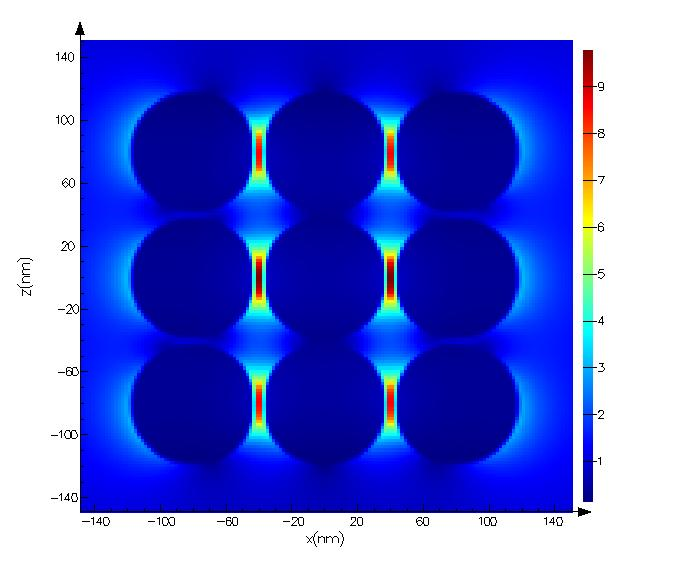
\includegraphics[width=0.95\textwidth]{fdtd-field-600nm}
  \end{minipage}
  %% \begin{minipage}[h]{0.49\textwidth} 
  %%   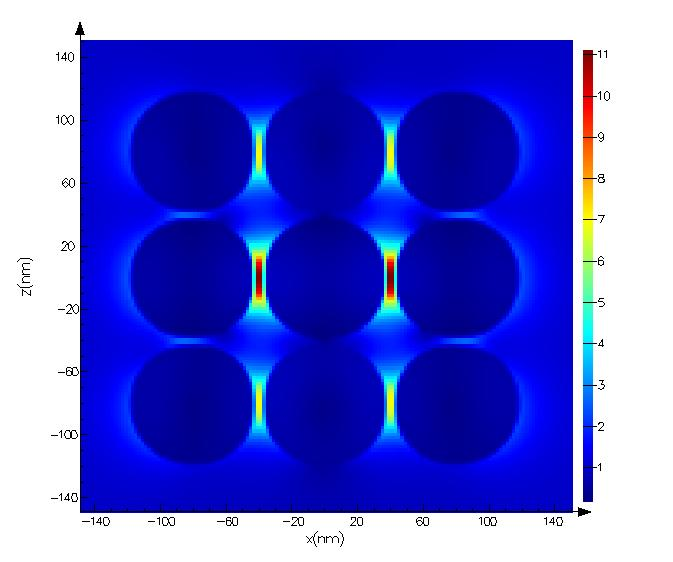
\includegraphics[width=0.95\textwidth]{fdtd-field-452nm}
  %% \end{minipage}
  
    \caption{ FDTD simulation of a 3x3 array of spheres, which are
      individually optimized for absorption at 525~nm(a) Fullwave
      simulation performed in Lumerical FDTD. (b) Cross-section
      absorption spectra (c,d,e) Field distribution for the
      wavelengths of 408, 452, and 600 nm.\label{fig:fdtd-3x3}}%
\end{figure}


\vspace{10pt}

\newpage
\begin{minipage}{1.0\linewidth}
  \textbf{Reviewer \#2 comments}\\
  \begin{tabular}[!H]{l|p{0.9\textwidth}}
    \quad & 1.  As we can find from the manuscript, the highest
    absorption efficiency is achieved for a Si/Ag core-shell
    structure, which is not located in the super absorbing
    regime. Moreover, the authors also claimed that from practical
    aspect, the core-shell structure (not in the super absorbing
    regime) could be easier and cheaper to fabricate than three
    layered structure (in the super absorbing regime). Therefore, the
    authors should clearly clarify what are the advantages or
    significances of the super absorption nanoparticles?
\end{tabular}
\end{minipage}

The super-absorption has a physical meaning of a regime, when we
create a structure, which has several highly absorbing resonances
overlapping in frequency, so that total absorption is larger than what
can be created in the structure with just one resonance. The main conclusions of the paper are
that a) We can create structures that shows superabsorption b) For
small particles (below 60nm), the efficiency of absorption is higher
in a single mode regime.  c) For larger particles the superabsorption
regime allows to achieve best efficiency of absorption.

To make this more clear in the manuscript, we have made the following changes to the manuscript: 

In the end of the first paragraph of page 3, right column, after
``..., since it should be easier and cheaper to fabricate.'' We add:
``At the same time the best absorption efficiency for larger particles
(with $R>60$~nm for provided materials) can be achieved in
superabsorption regime. This may be important when fabrication of
smaller multi-layer particles is not available.''


\begin{tabular}[!H]{l|p{0.9\textwidth}}
  \quad & 2.  In Fig. 2, we noticed a discontinuity at $\sim$80
  nm. The authors explain it as the design supporting electric dipole
  and magnetic quadrupole has larger ACS. However, this explanation is
  not clearly to me since it is lacking physics behind this
  phenomenon. The authors should clarify why the magnetic quadrupole
  only plays a significant role in this small wavelength range.
\end{tabular}

The short qualitative answer to this is that it is not possible to
excite the magnetic quadrupole resonance to the particle of a smaller
size, and, it is hard to make it absorb efficiently for larger sizes, while
also maintaining the large contribution of the electric dipole.

To present this idea in more details we run an optimization with
changed fitness function - we maximize the absorption efficiency of
only the electric dipole, with results presented in
Fig.~\ref{fig:a1max}. With the increase of the particle radius $R$, the electric dipole contribution
$\tilde{a}_1$ rapidly reaches its theoretical maximum. Optimizer was
quite successful in maintaining this for all larger values of $R$. When
we increase the $R$, other multipole resonances can appear. Such an
appearance of magnetic quadrupole term $\tilde{b}_2$ forms the discussed maxima at $\sim
80$~nm, and it is clearly observed in Fig.~\ref{fig:a1max}(b).

Another way to qualitatively explain the effect is the following. We
have a multiple resonance structure, and by changing parameters we can
overlap several different resonances. Depending on the total particle
size, different combination of resonances can give maximum absorption,
therefore it is not surprising that in a certain parameter range, the
combination of electric dipole and magnetic quadrupole can give us the
best possible absorption.

\begin{figure}
  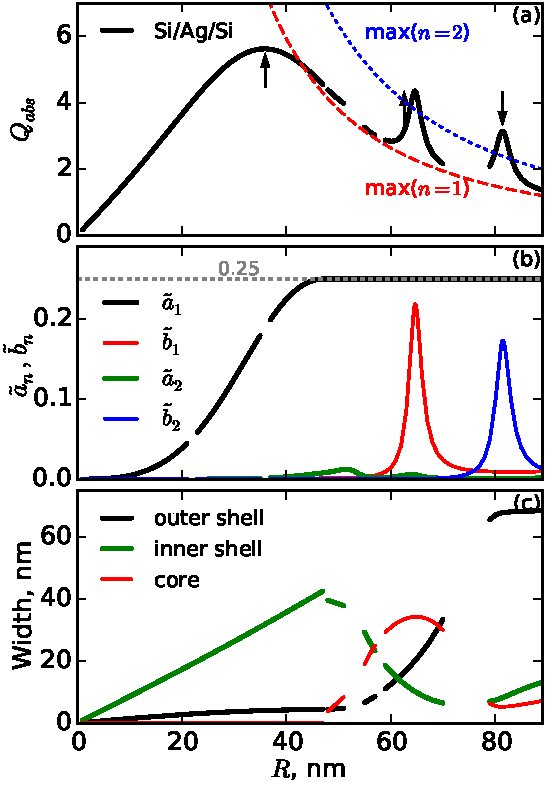
\includegraphics[width=0.35\textwidth]{overview-Qabs-a1}
   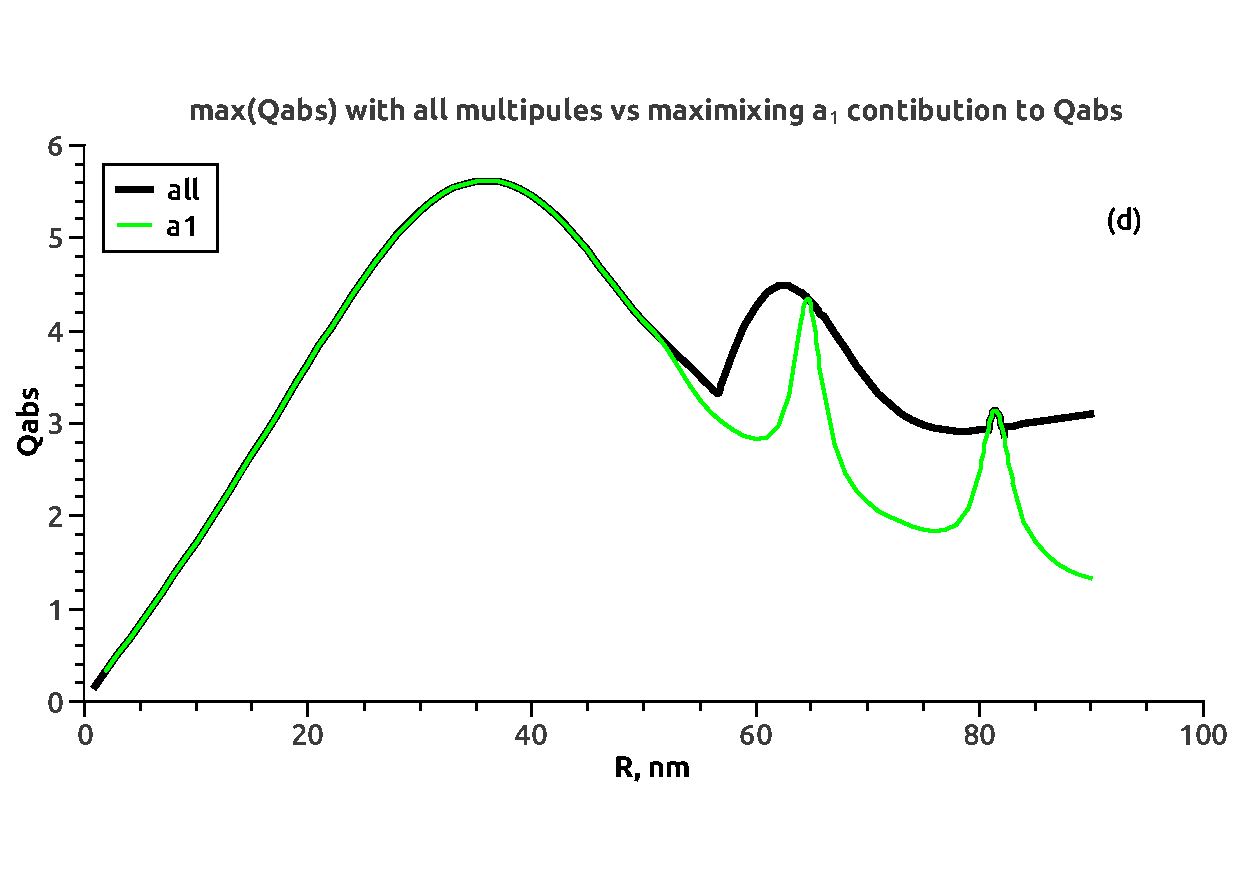
\includegraphics[width=0.60\textwidth]{overview-Qabs-all-a1}
  \caption{(a-c) Same as Fig.2 of the manuscript with different
    fitness function: the optimization aims to maximize the electric
    dipole absorption. (Missing points did not pass the stability
    test.) (d) $Q_{abs}$ for maximized $\tilde{a}_1$ from the first
    subplot of present figure without the additional stability test
    (green line) compared with $Q_{abs}$ optimization regarding all
    multipoles (black line, same as in Fig 2(a) of the
    manuscript).\label{fig:a1max}}
\end{figure}


\begin{tabular}[!H]{l|p{0.9\textwidth}}
\quad & 3.  In Fig. 3 (c), the authors observed a flat top of electric
dipole resonance. They attributed this flat resonance to the excited
several electric dipole resonances with close resonance
frequencies. Nevertheless, as we can see in Fig. 3 (d), even without
considering the resonances located in outer and inner shell, the
resonance inside the core is much broader than the other two
cases. The authors should explain this broadened resonance clearly.
\end{tabular}

We thank the referee for pointing this out, we must have not explained
this point clearly. The most interesting feature of this resonance
that we wanted to bring attention to is that the resonance has an
unusual flat top. The main shape and width of the resonance is
explained by one dominating dipole mode, as it is seen in the mode
decomposition in Fig.~3(d). Two additional electric dipole resonances
are much weaker, but their contribution "flattens" the top of the
combined absorption resonance. We have clarified this in the modified
manuscript changing the caption of Fig.~(3), after ``Panel~(d) shows
the superposition of the squared absolute values of the Mie
coefficients for electric dipole contribution inside each layer'' we
added ``of design from panel~(c), and it explains an almost
flat top of the electric dipole resonance.''


\begin{tabular}[!H]{l|p{0.9\textwidth}}
\quad & 4.  Some sentences are not clear to me. For instance, “there
is a strong conterplay between the increased absorption for larger
particles vs size for smaller particles”.  In summary, I do not think
the manuscript is acceptable at its current stage.
\end{tabular}%

We have worked on improving the readability of the
manuscript. Particularly, we changed the instance mentioned with the
reviewer, full sentence in the updated manuscript is now the
following: ``The absorption efficiency can be made large either by increasing ACS while keeping the particle size fixed, or by decreasing the particle size for fixed ACS. As a result, we show in this paper that smaller particles are more efficient when they operate in a single mode regime, while larger particles are more efficient absorbers when multiple modes are excited at the same frequency. ''
\end{document}
